\documentclass[10pt]{beamer}

\usetheme[progressbar=frametitle]{metropolis}
\usepackage{appendixnumberbeamer}
\usepackage{booktabs}
\usepackage[scale=2]{ccicons}
\usepackage{pgfplots}
\usepgfplotslibrary{dateplot}
\usepackage{xspace}
\usepackage{amsmath}
\usepackage{amsfonts}
\usepackage{graphicx}

\newcommand{\themename}{\textbf{\textsc{metropolis}}\xspace}

\usepackage{hyperref}

\title{Judging LLM-as-a-Judge}
\subtitle{Evaluating Chatbots using MT-Bench and Chatbot Arena}
\date{}
\author{Your Name} % Adjust the author name as needed
\institute{Your Institution} % Adjust institution

\begin{document}

\maketitle

% ============================================================
% TABLE OF CONTENTS
% ============================================================
\begin{frame}{Table of Contents}
  \begin{enumerate}
    \item The Core Problem
    \item Two New Benchmarks
    \item The Proposed Solution
    \item Unmasking the Biases (Limitations)
    \item Overcoming the Biases
    \item Does it Match Humans? (Agreement Study)
    \item Main Results \& Leaderboard
    \item A Hybrid Evaluation Paradigm
    \item Conclusion \& Open Source
  \end{enumerate}
\end{frame}

\section{The Core Problem}

\begin{frame}{Why Traditional Benchmarks Fail}
  \begin{itemize}
    \item Conventional benchmarks (MMLU, HELM) focus on \textbf{closed-ended, core knowledge tasks}.
    \item They \textbf{fail to capture} human preferences in \textbf{open-ended, multi-turn conversations}.
  \end{itemize}
  \vspace{0.3cm}
  % \begin{figure} 
  %    \centering
  %    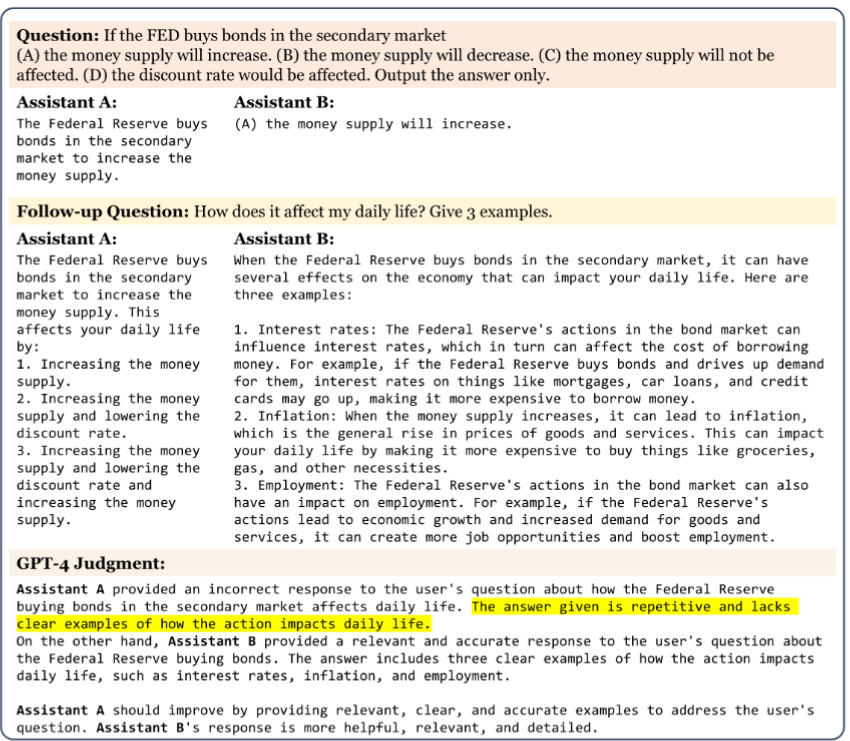
\includegraphics[width=0.7\textwidth]{images/1/figure1.png} 
  %    \caption{A multi-turn failure example.} 
  % \end{figure} 
  \textit{(Include Figure 1 showing multi-turn differences here.)}
\end{frame}

\section{Two New Benchmarks}

\begin{frame}{MT-Bench \& Chatbot Arena}
  \begin{itemize}
    \item \textbf{MT-Bench:} 80 high-quality, multi-turn questions across 8 core categories (Math, Coding, Writing, etc.).
    \item \textbf{Chatbot Arena:} Crowdsourced, anonymous chatbot battles in the wild (30K+ real-user votes).
  \end{itemize}
  \vspace{0.3cm}
   % \begin{figure} 
   %    \centering
   %    
\includegraphics[width=0.8\textwidth]{images/1/table1.png} 
   %    \caption{MT-Bench and Chatbot Arena Examples.} 
   % \end{figure} 
  \textit{(A snippet of Table 1 or a simple visual of MT-Bench vs. Arena works well here.)}
\end{frame}

\section{The Proposed Solution}

\begin{frame}{LLM-as-a-Judge}
  \begin{itemize}
    \item \textbf{Human evaluation} is the gold standard but too costly and slow.
    \item \textbf{Solution:} Use strong LLMs (like GPT-4) as a \textbf{scalable, explainable surrogate} to approximate human preference.
    \item \textbf{Three Judge Types:} 
    \begin{enumerate}
        \item Pairwise Comparison
        \item Single Answer Grading
        \item Reference-Guided Grading
    \end{enumerate}
  \end{itemize}
\end{frame}

\section{Limitations and Solutions}

\begin{frame}{Limitations \& Biases of LLM Judges}
  \begin{itemize}
    \item \textbf{Position Bias:} Favoring the first response position.
    \item \textbf{Verbosity Bias:} Favoring longer, wordy answers over concise ones.
    \item \textbf{Capability Flaws:} Struggling to accurately grade math and reasoning.
  \end{itemize}
  \vspace{0.3cm}
  % \begin{figure} 
  %    \centering
  %    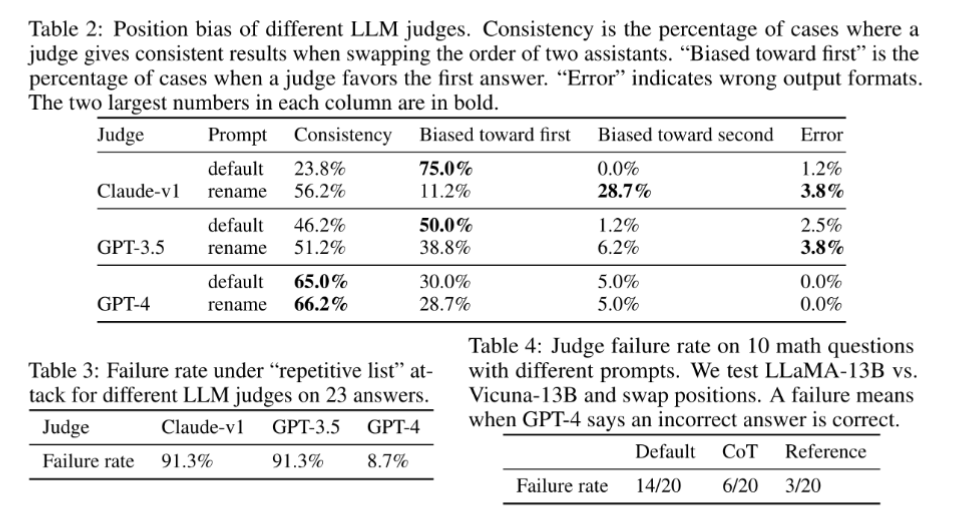
\includegraphics[width=0.7\textwidth]{images/1/table2.png} 
  %    \caption{Position bias across different LLM judges.} 
  % \end{figure} 
  \textit{(You can place Table 2 here to show position bias.)}
\end{frame}


\begin{frame}{Mitigating LLM Judge Limitations}
  \begin{itemize}
    \item \textbf{Swapping Positions:} Running comparisons twice and swapping order to \textbf{eliminate position bias}.
    \item \textbf{Chain-of-Thought (CoT):} Forcing the judge to solve the problem step-by-step first.
    \item \textbf{Reference-Guided Grading:} Providing a \textbf{baseline gold standard} answer to the judge.
  \end{itemize}
  \vspace{0.3cm}
  % \begin{figure} 
  %    \centering
  %    
\includegraphics[width=0.5\textwidth]{images/1/table4.png} 
  %    \caption{Math grading improves with references.} 
  % \end{figure} 
  \textit{(Place Table 4 here to show the drop in math failure rates.)}
\end{frame}

\section{Agreements and Results}

\begin{frame}{LLM Judges vs. Human Experts}
  \begin{itemize}
    \item GPT-4 achieves \textbf{>80\% agreement} with human experts.
    \item Matches the \textbf{exact agreement rate} found between human-to-human judges.
    \item Agreement scales higher when the performance gap between models is wider.
  \end{itemize}
  \vspace{0.3cm}
  % \begin{figure} 
  %    \centering
  %    
\includegraphics[width=0.6\textwidth]{images/1/figure2.png} 
  %    \caption{Agreement \% vs. Win Rate Difference.} 
  % \end{figure} 
  \textit{(Place Figure 2 here.)}
\end{frame}

\begin{frame}{Chatbot Performance Comparison}
  \begin{itemize}
    \item \textbf{Proprietary models} (GPT-4, Claude) significantly \textbf{outperform} open-source variants.
    \item Multi-turn benchmarks (Turn 2) \textbf{widen the gap} and better differentiate advanced models.
  \end{itemize}
  \vspace{0.3cm}
  % \begin{figure} 
  %    \centering
  %    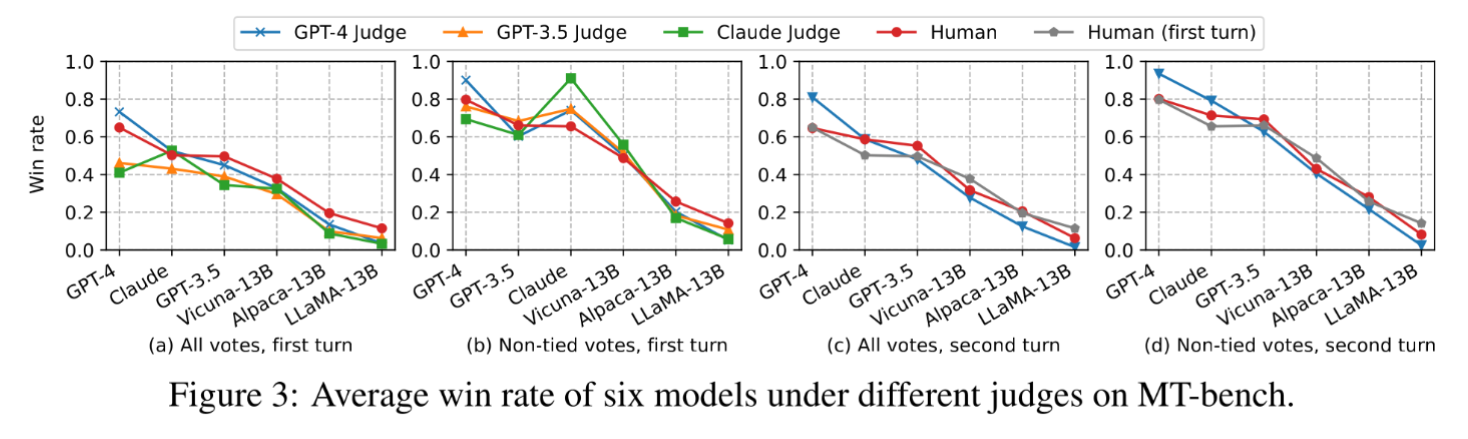
\includegraphics[width=0.7\textwidth]{images/1/figure3.png} 
  %    \caption{Win Rate curves comparing models.} 
  % \end{figure} 
  \textit{(Place Figure 3 or Figure 4 here.)}
\end{frame}

\section{Hybrid Paradigm \& Conclusion}

\begin{frame}{Standardized vs. Preference Benchmarks}
  \begin{itemize}
    \item No single benchmark tells the whole story.
    \item Fine-tuning on tiny datasets can \textbf{fake a "preferred style"} without improving core capabilities (MMLU).
    \item \textbf{Conclusion:} Future LLM evaluation must combine standard knowledge tests with LLM-as-a-judge preference benchmarks.
  \end{itemize}
  \vspace{0.3cm}
  % \begin{figure} 
  %    \centering
  %    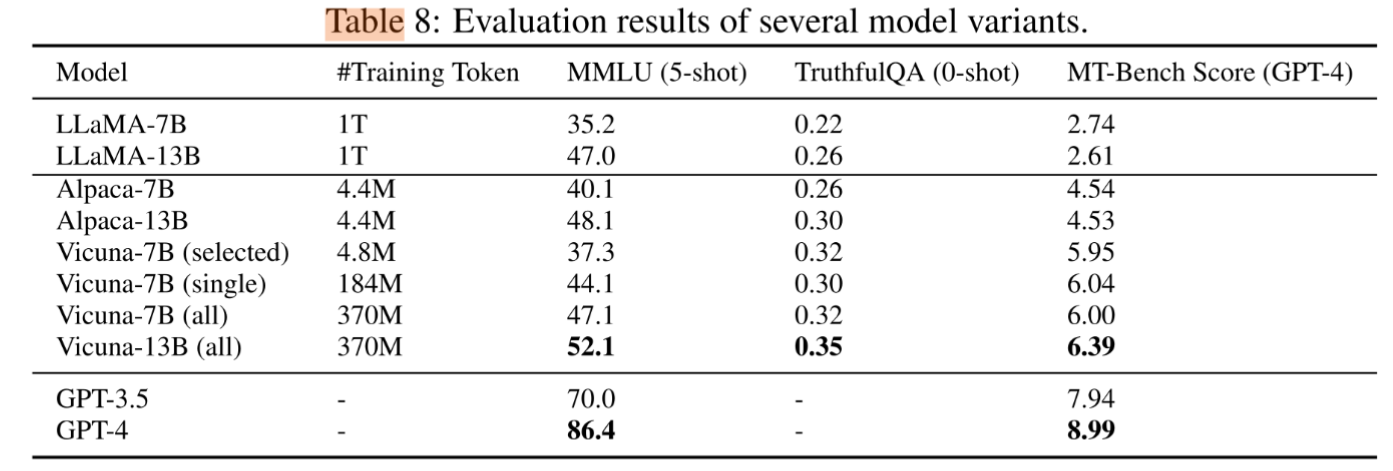
\includegraphics[width=0.6\textwidth]{images/1/table8.png} 
  %    \caption{Comparing traditional and preference benchmarks.} 
  % \end{figure}
  \textit{(Place Table 8 here.)}
\end{frame}

\begin{frame}{Key Takeaways}
  \begin{itemize}
    \item \textbf{LLM-as-a-judge} is a highly viable, scalable standard for the AI community.
    \item \textbf{Open-source judge models} (like fine-tuned Vicuna) show strong potential as cheap alternatives to GPT-4.
    \item \textbf{Publicly released:} 80 MT-bench questions, 3K expert votes, and 30K human conversations.
  \end{itemize}
\end{frame}

\end{document}
